\subsubsection{Set of subjects} \label{problem_scope_subjects}

Our dataset comprises considerably fewer documents than \acrshort{mag} (tens of thousands instead of hundreds of millions). Given that our goal is to relate documents to one another through their content, and we are focusing on small repositories, we don't require such granular subjects. If we used all the \acrshort{mag} subjects, most of them would be left unassigned, and many others would be assigned only once. We therefore pick a subset of these subjects.

\acrshort{mag} structures their set of subject as a hierarchy, where the first level comprises 19 subjects, which we call fields for clarity. Under each field, there exist five further hierarchy levels. We extract the subjects from OpenAlex, which is currently the best data source for subjects and publications of \acrshort{mag} (see section \ref{mag_access_data}).

In section \ref{problem_scope_subjects_retrieve}, we present our subject retrieval procedure. We discuss how many subjects we retrieve per field, and on what conditions we pick among the thousands of candidates. Then, we present the resulting set of subjects in section \ref{problem_scope_subjects_result}.

\paragraph{Subject retrieval} \mbox{} \label{problem_scope_subjects_retrieve}

We have extracted up to 200 descendants of each of the 19 fields. We consider how many publications a subject has been assigned to, assuming that popular subjects are more likely to appear in the repositories. We have tried different thresholds for how many assignments a subject needs to be considered, to strike a balance between picking subjects from the upper levels, which are more general, and picking subjects that are popular.

The problem is that the fields differ in popularity. For example, \textit{Medicine} has more than 200 subjects in the third level with more than 25k works, whereas \textit{Environmental science} only has 31 across all levels. We therefore start with a larger limit, iterate over all levels and all fields, and decrease the limit before iterating again. We first iterate through the descendants of each field and add subjects that are assigned to at least 25,000 publications. If the list of a field does not include 200 subjects after this iteration, we do so again, considering subjects assigned to at least 10,000. We repeat this procedure with 5,000, 1,000 and 100 assignments. When we iterate through the subjects of a field, we start by the second level and descend if necessary.

To avoid uninformative Wikipedia texts such as ``Emotionalism may refer to:'', we discard subjects whose description says ``Wikimedia disambiguation page'' or ``Wikimedia glossary list article''. The description from a subject comes from the corresponding Wikidata link, through which we later extract the Wikipedia link. For each subject that meets these requirements, we append it to all the fields it has in its list of ancestors, to keep the number of subjects as low as possible while providing good coverage of the fields.

\paragraph{Resulting set of subjects} \mbox{} \label{problem_scope_subjects_result}

\begin{figure}
    \centering
    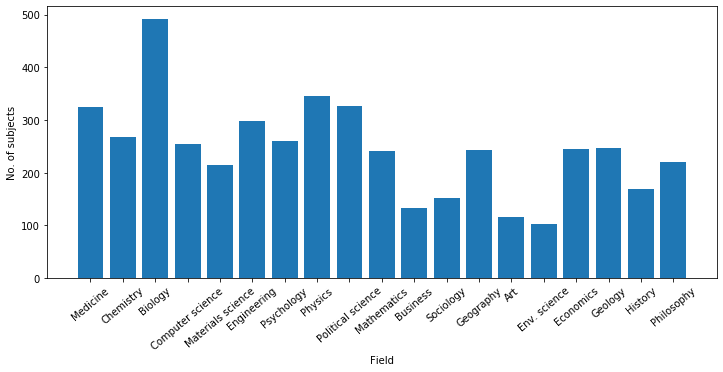
\includegraphics[width=\textwidth]{figures/unsupervised_approach/subjects_per_field.png}
    \caption{Number of subject that descend of each of the fields.}
    \label{fig:subjects_per_field}
\end{figure}

2,157 subjects were extracted with this procedure, which results on an average of 114 subjects per field. We could extract 200 subjects for all fields except for \textit{Environmental Science}, \textit{Business}, \textit{Sociology}, \textit{Art} and \textit{History}. On the other hand, \textit{Medicine}, \textit{Biology} and \textit{Physics} have more than 300 descendant subjects under the ones we have collected. This is because subjects can descend from multiple fields. For example, \textit{Neuroscience} can be classified under \textit{Biology}, \textit{Medicine} and \textit{Computer science}. The number of subjects per field can be seen in figure \ref{fig:subjects_per_field}.

All 25 subjects of the second level have been picked, followed by 1,999 of the third level, 108 of the fourth, and 6 of the fifth. On average, subjects are assigned to 197,180 publications. No subjects are assigned to less than 100 documents, as this was a requirement in the extraction procedure. Regarding the hierarchy of the subjects, all but 13 of them have ancestors in all levels above them. Two subjects of the third, \textit{Sensitivity} and \textit{Boundary}, are directly linked to fields. \textit{Sensitivity} is a descendant of both \textit{Engineering} and \textit{Mathematics}, whereas \textit{Boundary} descends from \textit{Mathematics}. The remaining eleven subjects that don't have ancestors in all previous levels belong to the fourth level. All of them descend from subjects of the second level, thus skipping the third level.